\chapter{Methods}

\section{Our Model}

Our model is based on the classic Wright-Fisher [3][4] and Stepping-Stone [5] population genetic models which describe evolution and migration, respectively. The model describes the allele frequency in a population of N individuals grouped into discrete \textit{demes}, or subpopulations, connected by migration (Figure \ref{fig:schematic}). 

\begin{figure}[h]
    \centering
    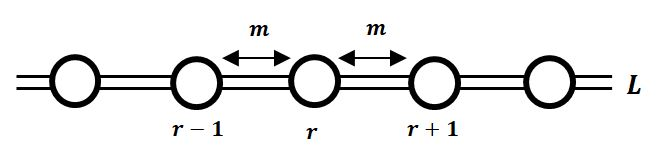
\includegraphics[scale=0.8]{img/model_schematic.JPG}
    \caption{This schematic represents the geographic structure for the model in one dimension. Circles represent demes which are indexed by integer $r$. There are $L$ many demes connected to nearest neighbors via a symmetric migration rate $m$. The boundaries are connected to one another, effectively creating a \textit{ring} of demes.}
    \label{fig:schematic}
\end{figure}
	

The model simplifies the system by considering a single genetic locus with two alleles. The allele frequency in each deme, $f_r$, evolves due to four forces:


\begin{enumerate}
    \item \textbf{Mutation} changes one allele to another at rate $\mu$
    \item \textbf{Natural selection} reduces the frequency of the deleterious allele at rate $s$
    \item \textbf{Genetic drift} introduces random noise in a finite population at rate $\frac{1}{N}$, \\ where $N$ is the population size
    \item \textbf{Migration} reduces the allele frequency differences between nearby demes at rate $m$
\end{enumerate}

\newpage
The change in allele frequency at each deme due to these forces is described by the stochastic differential equation:
\begin{equation}
    \label{eq:model}
    df_r=[\mu(1-2f_r)-sf_r (1-f_r ) + m (f_{r-1}+f_{r+1}-2f_r)]dt+\sqrt{\frac{f_r (1-f_r )}{N}} dB_{t,r}
\end{equation}


While these models have been studied extensively [14][15][16], most work has been focused on neutral evolution. Expanding the Wright-Fisher model allows us to examine allele frequencies acted upon by each of the four evolutionary forces. We simulate the evolution of rare deleterious alleles over many generations and over large geographic environments. Using this equation, important information about the evolution of rare deleterious alleles can be discovered. In the next chapter, we will derive important quantities that describe the average number of rare allele copies as a function of the evolutionary parameters along with the quantity describing the average geographic range of an allele. We will describe the equilibrium distribution of allele frequencies across demes.


Our approach involves first simulating the underlying distribution of allele frequencies, and second, sampling from this distribution using a variety of sampling scheme. Our subsequent analysis examines the information loss as a function of sampling. We are interested in the interaction between the process of sampling and the "unobserved" underlying frequency distribution. 

\begin{figure}[h]
    \centering
    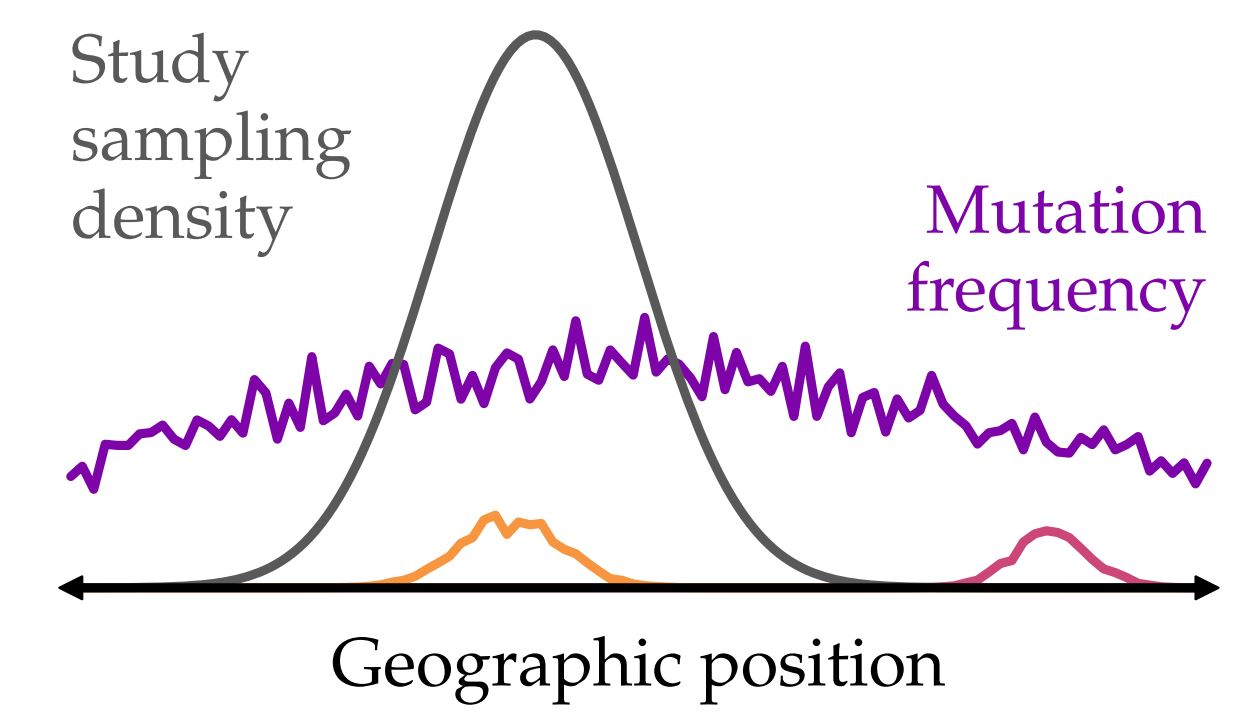
\includegraphics[scale=0.5]{img/smapling_schematic.JPG}
    \caption{This schematic illustrates the interaction between the underlying allele frequency distribution and the sampling scheme imposed by an association study. We see that alleles are typically confined to a range of geographic positions, and we expect the alleles sampled in a study to depend on where the sampling distribution is relative to the allele frequency distribution.}
    \label{fig:sampling_schematic}
\end{figure}

\newpage
\section{Simulating Spatial Evolution}




\section{Introducing Sampling Effects}

